\chapter{开发周期}


    \section{如何合作开发?}

        \subsection{开发环境}
        Leap Motion官方Python2 SDK, 具体的环境说明以及配置方法见Git仓库的README。

        \subsection{设计分工}
        使用了观察者模式,ChordHandler, StrummingHandler分别处理Leap motion到来的帧\
        分开左手与右手的处理,并且不用修改主程序。

        使用了组合,一个吉他模拟器Guitar实例将提供set\_chord, play\_string方法,使\
        处理输入数据后可以方便地改变吉他的状态。

    \section{如何迭代开发?}

        使用Git作为版本控制和分支管理的工具,任务分配通过GitHub上的Issue功能开展。\
        Merge Request组员都会收到并且互相进行Code Review,使我们代码质量较高、\
        开发进度也一直较快,在阶段展示的时候完成度就已经非常高。

        由于设备只有一台,故大多数时候其实并不能并行开发。
        
        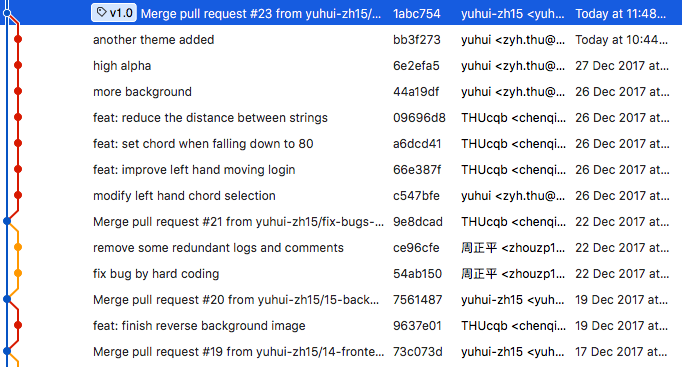
\includegraphics[width=\textwidth]{git}
